\chapter{image}



\section{image\_Quadricycle First Edition}
41023230機器人\\
\begin{figure}
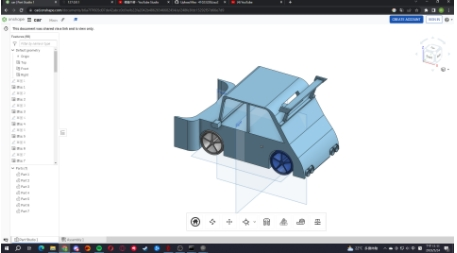
\includegraphics[width=3.75in]{41023230robot1}
\end{figure}
41023231機器人\\
\begin{figure}
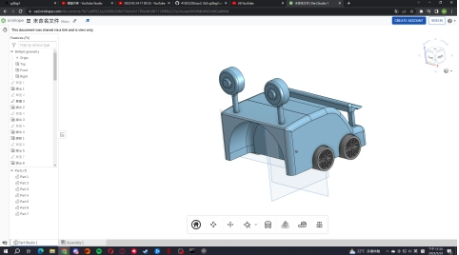
\includegraphics[width=3.75in]{41023231robot1}
\end{figure}
41023232機器人\\
\begin{figure}
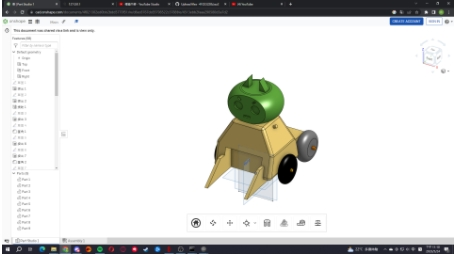
\includegraphics[width=3.75in]{41023232robot1}
\end{figure}
41023233機器人\\
\begin{figure}
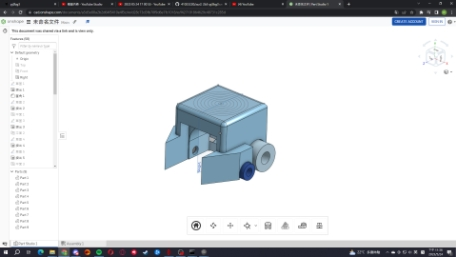
\includegraphics[width=3.75in]{41023233robot1}
\end{figure}
41023253機器人\\
\begin{figure}
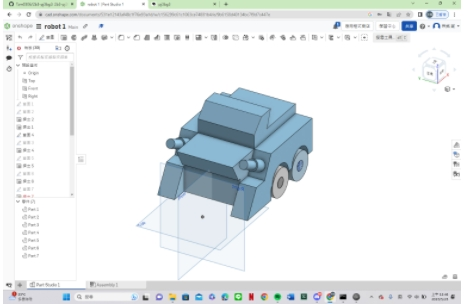
\includegraphics[width=3.75in]{41023253robot1}
\end{figure}
\section{image\_Quadricycle Second Edition}
41023233機器人\\
\begin{figure}
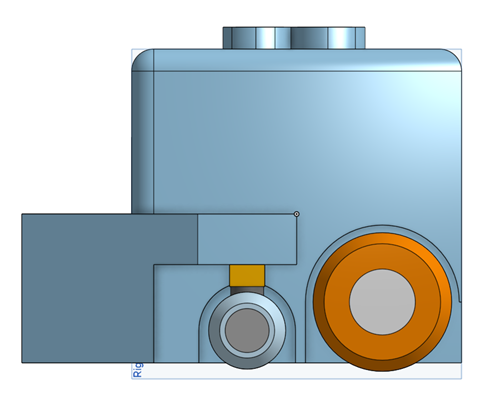
\includegraphics[width=3.75in]{41023233robot2}
\end{figure}
41023250機器人\\
\begin{figure}
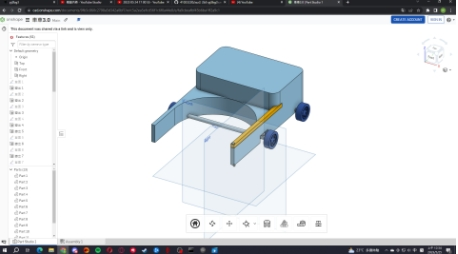
\includegraphics[width=3.75in]{41023250robot2}
\end{figure}
\section{image\_court}
球場本體\\
\begin{figure}
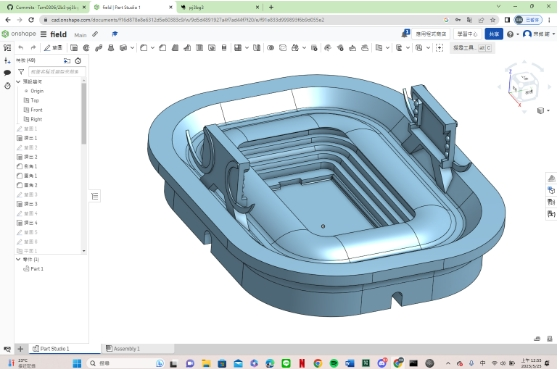
\includegraphics[width=3.75in]{court}
\end{figure}
球門\\
\begin{figure}
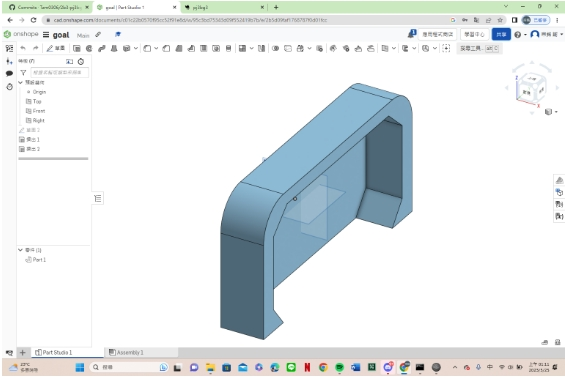
\includegraphics[width=3.75in]{goal}
\end{figure}
球場球門組合\\
\begin{figure}
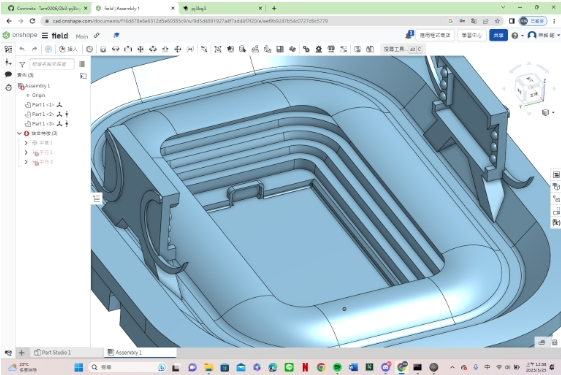
\includegraphics[width=3.75in]{court+goal}
\end{figure}
組合並加入車子\\
\begin{figure}
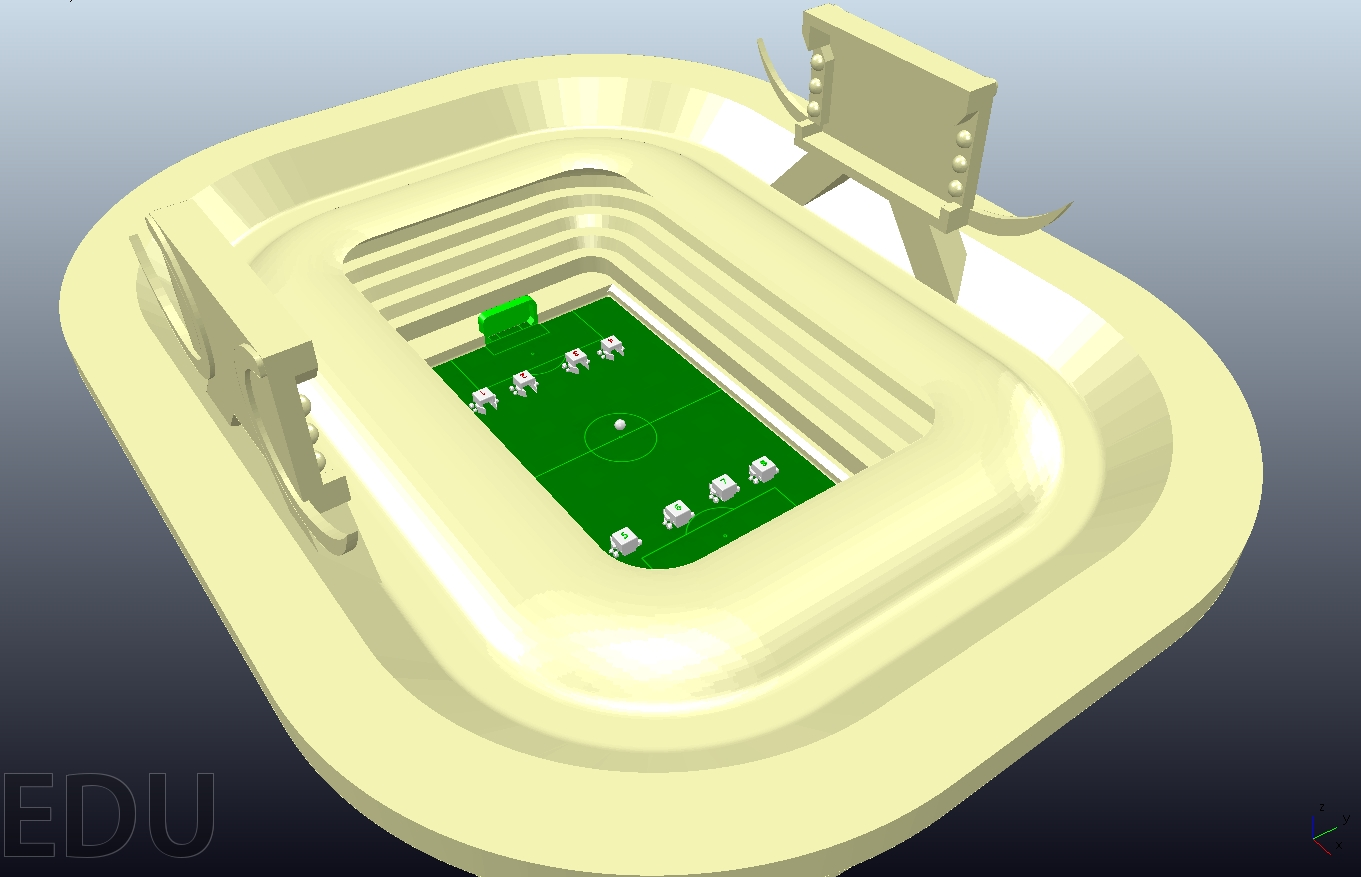
\includegraphics[width=3.75in]{race}
\end{figure}
可修改方向:將球場獨立出來,如此可把觀眾席設為non-respondable,使其模擬時速度增加。\\
經修改後的獨立球場\\
\begin{figure}
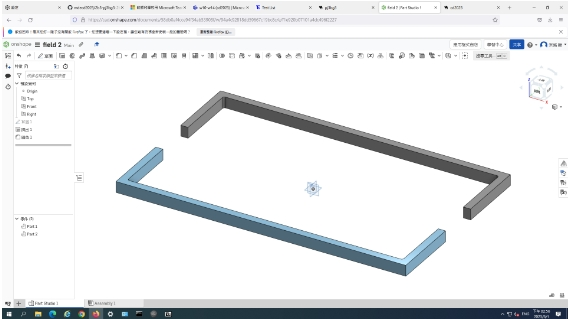
\includegraphics[width=3.75in]{Independence Stadium}
\end{figure}
\section{image\_race}
\begin{figure}
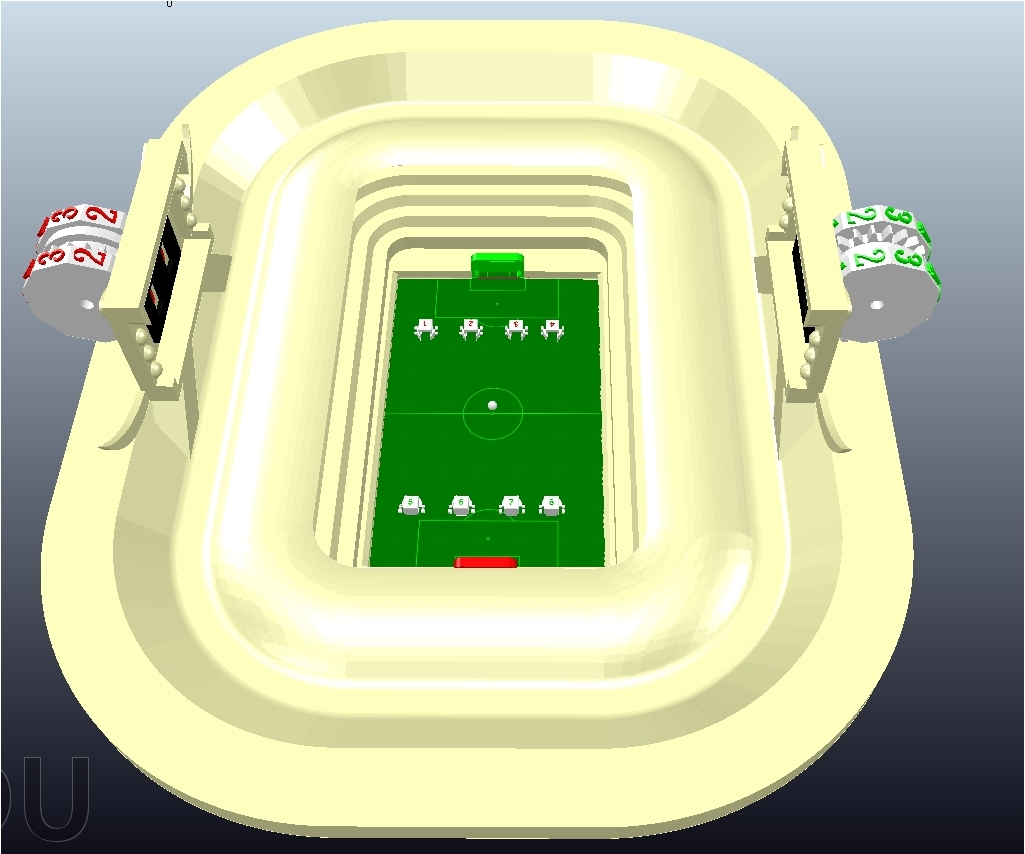
\includegraphics[width=5in]{race2}
\end{figure}


